\section{Methods}

We use two atmospheric models to estimate the atmospheric changes: the first is a simple one-dimensional model of a convective boundary layer, and the second is a complex three-dimensional regional climate model.  Because of their differing levels of complexity, these models have complementary strengths and weaknesses.  The simple model isolates the central physical processes of land surface energy partitioning and entrainment of free tropospheric air; however, the simple model neglects secondary but important processes such as lateral advection, topographic effects on flow, and radiation change.  The complex model, on the other hand, includes these and many other processes and can thus represent spatial heterogeneity and unanticipated feedbacks; however, the inclusion of so many processes can obscure the connection between stomatal dynamics and temperature and humidity changes.  By using both models, we test the robustness of the stomatal effects and explore both the central processes and the complex implications.

In both models, we use the stomatal response parameters for soil moisture and $VPD$ derived in the previous chapter to calculate stomatal conductance and thus latent heat flux.  Tests with each model are conducted over a range of soil moisture values and synoptic conditions typical of August in the northern California Coast Range.  We quantify the differences in surface temperature, near-surface air temperature, boundary layer depth, and near-surface humidity between a hypothetical all-Douglas-fir forest and a hypothetical all-Pacific-madrone forest.

\subsection{1-D model}
The 1-D model [\cite{tennekes1981basic}; \textit{Garratt}, 1992 XXXX; \cite{Siqueira:2009qf}] simulates the evolution of boundary layer height, potential temperature, and humidity, given surface fluxes and free troposphere conditions.  The boundary layer is assumed to be well mixed, with uniform potential temperature ($\Theta$, Kelvin) and specific humidity ($Q$, g/kg), and to be capped by a temperature inversion represented by a step change, as shown in Figure 2 from \cite{Siqueira:2009qf}.  The height of the boundary layer, $h$ (m), is assumed to grow due to buoyant convection only, in such a way that the entrainment heat flux at the top of the boundary layer is a fixed fraction of the sensible heat flux at the land surface (as in \textit{Garratt} [1992] XXXX, Section 6.1.5.)  Because the model is 1-D, it assumes horizontal homogeneity, meaning no lateral variation in surface fluxes or properties and no net horizontal advection.

The evolution of $h$ is modeled as

% dh/dt equation
\begin{equation}
\frac{dh}{dt} = (1+2\beta)\frac{H/\rho c_p}{\Gamma_\Theta h},
\label{eqn:dhdt}
\end{equation}
where $H$ is the surface sensible heat flux (W/m$^2$), $\rho$ is the density of air (kg/m$^3$), $c_p$ is the heat capacity of air at constant pressure (J/kg/K), $\Gamma_\Theta$ is the lapse rate of potential temperature above the boundary layer (K/m), and $1+2\beta$ is the proportionality relating surface sensible heat flux to entrainment heat flux at the top of the boundary layer.  The time tendency of the boundary layer height, and thus of entrainment at the top of the boundary layer, is used to solve for the evolution of $\Theta$ and $Q$:

% dTheta/dt equation
\begin{equation}
\frac{d\Theta}{dt} = \frac{1}{h}\left(\frac{H}{\rho c_p}+\Delta\Theta\frac{dh}{dt}\right)
\label{eqn:dTdt}
\end{equation}
% dQ/dt equation
\begin{equation}
\frac{dQ}{dt} = \frac{1}{h}\left(\frac{E}{\rho}+\Delta Q \frac{dh}{dt}\right),
\label{eqn:dQdt}
\end{equation}
where $E$ is surface evapotranspiration (g/m$^2$/s), $\Delta\Theta$ (K) is the jump in potential temperature across the inversion at the top of the mixed layer, and $\Delta Q$ (g/kg) is the jump in specific humidity across the inversion.  These jumps are calculated using

% dDTheta/dt equation
\begin{equation}
\frac{d\Delta\Theta}{dt} = \Gamma_\Theta\frac{dh}{dt}-\frac{d\Theta}{dt}
\label{eqn:dDTdt}
\end{equation}
% dDQ/dt equation
\begin{equation}
\frac{d\Delta Q}{dt} = \Gamma_Q\frac{dh}{dt}-\frac{dQ}{dt},
\label{eqn:dDQdt}
\end{equation}
where $\Gamma_Q$ is the lapse rate of water vapor above the mixed layer.

$E$ is the sum of transpiration ($E_t$) and soil evaporation ($E_{soil}$); evaporation of intercepted canopy water is negligible during the dry season days considered here.  $E_t$ is simulated following the procedure in Section \ref{sec:sapflow_regmeth}: normalized sap velocity at the outer edge of the sapwood ($v_n$, ranging from 0 to 1) is predicted with a Jarvis model for stomatal conductance [\cite{jarvis1976interpretation}] with parameters estimated from sap flow measurements (species-averaged parameters in Table \ref{tbl:sapflow_maxvel}), and $v_n$ is scaled up to regional transpiration using the observed Douglas fir tree-diameter--sapwood-depth relationship (Equation \ref{eqn:sapwood}`) and an FIA-derived tree size distribution [\textit{Woudenberg et al.}, 2010 XXXX, all-species distribution, black line in Figure \ref{fig:sapflow_abundances}].  The Douglas fir sapwood depth relation is used for both the Douglas fir and Pacific madrone model runs in order to eliminate variation due to sapwood area and focus on variation due to stomatal response.

Soil evaporation is estimated using a simplified version of the CLM model soil evaporation scheme [\cite{oleson2010technical}]:
\begin{equation}
E_{soil} = \frac{-\beta_{soi}(q_{air}-q_{ground})}{r_{aw}+r_{litter}},
\end{equation}
where $\beta_{soi}$ is a reduction factor based on soil moisture (Equation 5.68 in \cite{oleson2010technical} with $\theta_{fc,1}=0.15$), $q_{air}$ is the specific humidity of the air (g/kg), $q_{ground}$ is the saturation specific humidity at ground temperature (g/kg), $r_{aw}$ is the resistance to water vapor transfer from the ground to the canopy air space (Equation 5.99 in \cite{oleson2010technical} with $C_s=0.004$ and $u_*=0.4$ m/s), and $r_{litter}$ is the resistance to water vapor transfer through the litter layer (Equation 5.106 in \cite{oleson2010technical} with $L^{eff}_{litter}=0.5$ m$^2$/m$^2$).

Incoming radiation is prescribed using typical values for August in this region.  For incoming solar radiation ($S_{down}$), we use the average diurnal course of total solar radiation measured at an open meadow station at the Angelo Coast Range Reserve (ACRR) on August 15 of 2009-2011.  For downward longwave radiation ($L_{down}$), we use the GEWEX Surface Radiation Budget [Stackhouse \textit{et al.}, 2011 XXXX] mean diurnal pattern from the month of August (years 2003-2007) for the grid cell nearest the ACRR field site.  Shortwave albedo is set to 0.1 and longwave emissivity is set to 0.95 for both species in order to eliminate variation due to vegetation radiative properties (0.1 is the albedo and XX is the emissivity for broadleaf evergreen temperate trees in CLM [\cite{oleson2010technical}].)  Ground heat flux is set equal to 5\% of net radiation [\cite{ogee2001long}].  Aerodynamic resistance ($r_a$) is held constant at 10 s/m, which is a representative value for typical winds and near neutral conditions using Equation 14.33 from \cite{bonan}; this particular value was chosen to give surface and air temperatures close to observations.

Given this predicted $E$, along with prescribed incoming radiation and aerodynamic resistance, the surface energy balance is solved for surface temperature ($T_s$, K) using the Newton-Raphson method and a timestep of 1 second, and $T_s$ is then used to calculate outgoing longwave radiation ($L_{up}$, W/m$^2$) and sensible heat flux ($H$, W/m$^2$).  Potential temperature $\Theta$ is adjusted for altitude to air temperature $T_a$ for calculating $H$ and $LE_t$ (VPD), using an altitude of 400 m and an adiabatic lapse rate of 10 K/km.  

Free troposphere conditions (needed for $\Gamma_{\Theta}$ and $\Gamma_Q$ in Equations \ref{eqn:dhdt}, \ref{eqn:dDTdt}, and \ref{eqn:dDQdt}) are derived from atmospheric soundings at Oakland International Airport, 250 km south of the Rivendell field site (downloaded from the archive at the University of Wyoming, \url{http://weather.uwyo.edu/upperair/sounding.html}).  The sounding site and field site are similar distances from the Pacific coast (16 km for the field site and 25 km for Oakland Airport) and both have prevailing wind directions from the west over the ocean.  Oakland is influenced by fog, but it is also at lower altitude (near sea level), whereas much of northern Coast Range forest region has a base elevation of at least 400 m; as such, we neglect sounding measurements from below 400 m, thus excluding much of the fog.  Profiles of $\Theta$ and $Q$ from 4 AM local time are averaged for the months of July and August from 2009 to 2011, binned by daily maximum temperature ($T_{max}$) measured at the ACRR: cool days ($T_{max} < 20^{\circ}$C), intermediate days ($20^{\circ}$C $\le T_{max} < 30^{\circ}$C), and hot days ($T_{max} \ge 30^{\circ}$C).  The average profiles and the piecewise linear approximations used in the model are shown in Figure \ref{fig:BL_LapseRates}.

\begin{figure}[here]
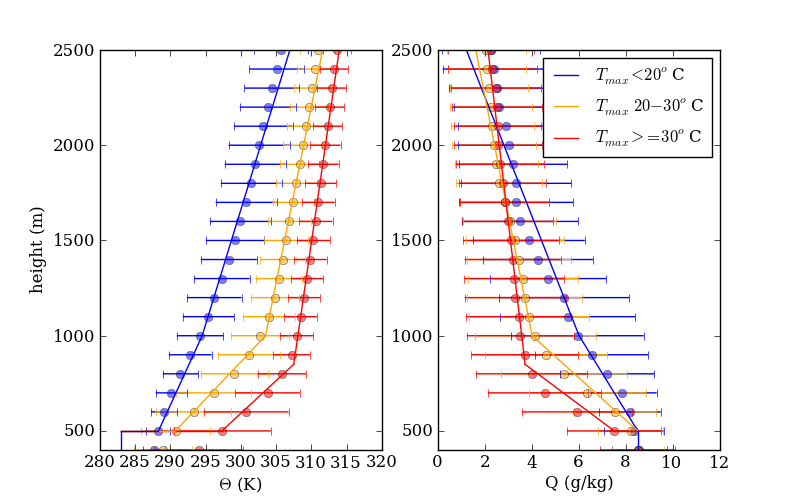
\includegraphics[width=1\textwidth]{ch2-BL/figures/fitted_lapserates_theta_Q_onefig.png}
\caption{Symbols: potential temperature ($\Theta$, left) and specific humidity ($Q$, right) from Oakland Airport soundings at 04:00 local time, averaged for July and August 2009-2011 and binned by height.  Error bars show one standard deviation.  Lines: piecewise linear approximations to the lapse rates for $\Theta$ and $Q$, which are used in the 1-D boundary layer model.}
\label{fig:BL_LapseRates}
\end{figure}

The range of soil moisture, free troposphere, and tree species conditions tested are listed in Table \ref{table:BL_1Druns}.  

\begin{table}
\begin{tabular}{ l c }
\hline
 & Range of values tested \\ \hline
Jarvis $VPD$ and $\theta_{rel}$ parameters & Douglas fir, Pacific madrone (Table XXX)\\
Lapse rates $\Gamma_{\Theta}$ and $\Gamma_Q$ & 1 (blue in Figure \ref{fig:BL_LapseRates}), 2 (yellow), 3 (red)\\
Relative soil moisture $\theta_{rel}$ & 0.15, 0.2, 0.25, 0.3, 0.35, 0.4, 0.45, 0.5\\
\hline
\end{tabular}
\caption{Range of values tested using the one-dimensional boundary layer model.}
\label{table:BL_1Druns}
\end{table}

\subsection{Regional climate model}
\label{sec:BL_WRFdesc}
In order to further test the impact of these two tree species on the atmospheric boundary layer, we use WRF-Noah [Skamarock \textit{et al.}, 2008], a three-dimensional, non-hydrostatic regional climate model (Weather Research and Forecasting, or WRF) with terrain-following vertical coordinates and a coupled land surface model (Noah).  In WRF, the conservation equations for momentum, mass, and energy are solved numerically to calculate the temporal evolution of atmospheric state variables, including air temperature, pressure, humidity, and wind velocity.  WRF has a range of parameterization options for radiation, turbulence treatment via planetary boundary layer (PBL) schemes or large-eddy simulation closures, cloud microphysics, convection, bottom boundary fluxes of water vapor and heat, and lateral boundary forcing.  

\begin{table}
\begin{tabular}{l l}
\hline
Scheme & Setting \\ \hline
WRF version & 3.6 \\
Grid nesting & two-way \\
Lateral boundary conditions & NCEP Eta analysis \\
Soil levels & 4 \\
Land use and soil categories & USGS \\
Land surface model & Noah \\
Surface layer & MM5 Monin-Obukhov \\
Planetary Boundary Layer (PBL) & ACM2 \\
Microphysics & WSM 3-class simple ice \\
Longwave radiation & RRTM \\
Shortwave radiation & Dudhia \\
Cumulus & Kain-Fritsch (new Eta) \\
Turbulence closure & Horizontal Smagorinzky first order \\
Momentum advection & 5th order horizontal, 3rd order vertical \\
Scalar advection & Positive definite \\
Lateral boundary & 5 grid points \\
\hline
\end{tabular}
\caption{WRF parameterization options.  See Skamarock \textit{et al.} [2008] for description of schemes.}
\label{table:BL_paramschemes}
\end{table}

The parametrization schemes used here are listed in Table \ref{table:BL_paramschemes}.  Most schemes chosen are the default settings for realistic (non-idealized) simulations, with the exception of the ACM2 PBL scheme. The ACM2 scheme is used because of its ability to represent both convective regimes (non-local transport) and shear-dominated regimes (local transport) [Pleim, 2007], and because of its good performance in other WRF studies [CITATIONS including Marjanovic].

\begin{table}
\begin{tabular}{ l c c c c c c c }
\hline
Domain & $\Delta x$ (km) & $\Delta y$ (km) & $nx$ & $ny$ & $nz$ & $\Delta t$ (s) & USGS data res \\ \hline
d01 & 8.1 & 8.1 & 96 & 99 & 45 & 45 & 2 min\\
d02 & 2.7 & 2.7 & 175 & 175 & 45 & 15 & 2 min\\
\hline
\end{tabular}
\caption{Model domains. d01 refers to the outer domain, and d02 refers to the inner domain.}
\label{table:BL_domains}
\end{table}

\begin{figure}[here]
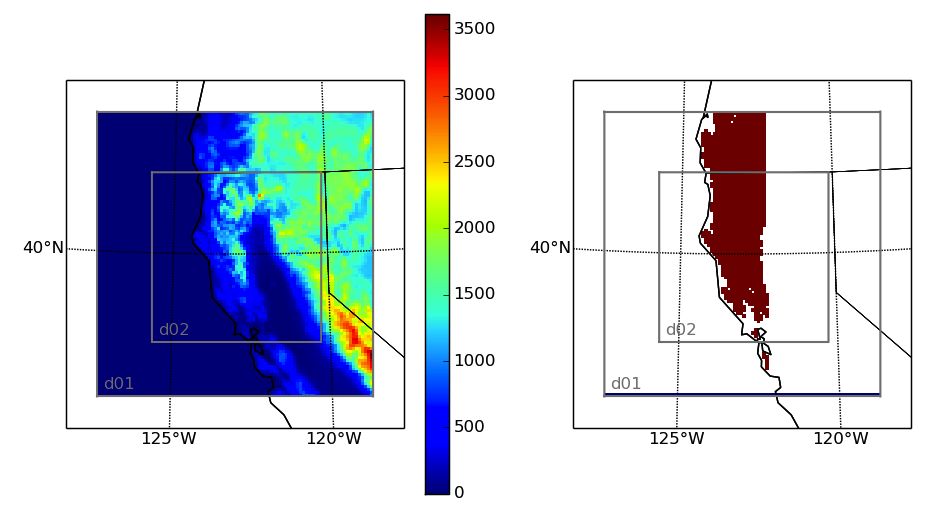
\includegraphics[width=1\textwidth]{ch2-BL/figures/domain_map_cropped.png}
\caption{WRF domains over northern California.  The gray outlines show the domain boundaries; d01 is the outer nest, and d02 is the inner nest.  Left: topographic elevation; right: red shows the test region where vegetation parameters are modified.}
\label{fig:BL_domain}
\end{figure}

The tests are run with two nested domains centered on the northern Coast Range (Figure \ref{fig:BL_domain}).  The use of two nests enables gradual down-scaling of the coarse lateral forcing to the high resolution needed to resolve flow over the Solano wind farm.  We adopt a conservative nesting grid ratio of 3:1.  The outer domain (d01) provides the lateral boundary conditions for the inner domain (d02), and the inner domain states are fed back to the outer domain throughout the region coincident with the inner domain.  Two-way nesting increases model accuracy, particularly in regions of complex terrain [CITATIONS].  The domain resolutions and dimensions are listed in Table \ref{table:BL_domains}.  The lateral boundaries of the outer domain are forced with NCEP Eta 212 grid (40 km) operational analysis [NCEP, 1998] for the period of 2009-08-16 00:00 to 2009-08-30 00:00, with the first 32 hours discarded as model spin-up.  This time period is rain-free and sunny at the Angelo Reserve and represents the mid- to late-summer season when soil is very dry and incoming radiation is still strong (cf. Chapter \ref{c.sapflow} Figure XX - rivendell met time series).

The two hypothetical forests (all-Douglas-fir and all-Pacific-madrone) are tested in the northern Coast Range region highlighted in Figure XX.  In this region, dummy land use and soil types are used, and the VPD and soil moisture stomatal response parameters of this dummy type are modified according to the test case, as described below.  Radiative properties, leaf area, and rooting depth of the dummy type are held constant among the test cases, using the ``Evergreen Needleleaf Forest'' values.  Outside of the test region, observed topography and USGS vegetation and soil types are used.

\begin{table}
\begin{tabular}{ l p{3cm} p{3cm} p{2cm} p{3cm} }
\hline
Vegetation type & $\theta_{ref}$ (m$^3$/m$^3$) & $\theta_{wilt}$ (m$^3$/m$^3$) & $RS$ (s/m) & $HS$ (kg/kg)\\ \hline
%ENF & 0.329 (loam) & 0.066 (loam) & 125 & 47.35\\
Douglas fir & 0.156 & 0.075 & 125 (ENF) & 47.35 (ENF)\\
%EBF & 0.329 (loam) & 0.066 (loam) & 150 & 41.69\\
Pacific madrone & 0.105 & 0.047 & 150 (EBF) & 41.69 (EBF)\\
%Pacific madrone 2 & 0.105 & 0.047 & 300 & 20.\\
\hline
\end{tabular}
\caption{Parameters for Noah's Jarvis formulation of stomatal conductance, by vegetation type.  $RS$ is the Noah minimum stomatal resistance parameter in the Jarvis formulation. $HS$ is the Noah scaling factor for the specific humidity deficit in the Jarvis humidity stress function (Equation XX).  ENF is the USGS Evergreen Needleleaf Forest land use type; EBF is the USGS Evergreen Broadleaf Forest land use type.}
\label{table:BL_NoahJarvisparams}
\end{table}

\begin{table}
\begin{tabular}{ l p{6cm} p{7cm} }
\hline
Run ID & VPD parameters ($RS$, $HS$) & Soil moisture parameters ($\theta_{ref}$, $\theta_{wilt}$)\\ \hline
vDF-sDF & Douglas fir (ENF) & Douglas fir\\
%vEBF-sMD & EBF & Pacific madrone\\
vMD-sMD & Pacific madrone (EBF) & Pacific madrone\\
%vMD2-sMD & Pacific madrone 2 & Pacific madrone\\
\hline
\end{tabular}
\caption{Combinations of stomatal conductance Jarvis parameters used in the WRF tests.  Each pair of parameters is tested for a range of volumetric soil moisture values in the northern Coast Range test region: 0.08, 0.1, 0.12, and 0.14 m$^3$/m$^3$.}
\label{table:BL_WRFruns}
\end{table}

The test region stomatal conductance parameters are modified to quantify the differences between the hypothetical all-Douglas-fir and all-Pacific-madrone cases.  The Noah model uses a Jarvis formulation of stomatal conductance similar to that used in Chapter \ref{c.sapflow} (Equation XX).  The $RS$ parameter is the minimum stomatal resistance (equivalent to $1/g_{s,max}$), and $RS$ is divided by empirical functions of environmental variables to give the actual stomatal resistance.  

The soil moisture stress function is the piecewise-linear, threshold Feddes model [\textit{Feddes et al.}, 1978; \textit{Chen et al.}, 2008].  The parameters for the sigmoid model from Chapter \ref{c.sapflow} (Equation XX, Table XX) thus must be translated to the Feddes parameters (reference or stress point, $\theta_{ref}$, and wilting point, $\theta_{wilt}$).  For each species, we fit a line to $f_{\theta}$ between $f_{\theta}=0.05$ and $f_{\theta}=0.95$ and extrapolate the line to 0 to estimate $\theta_{wilt}$ and to 1 to estimate $\theta_{ref}$ (Figure \ref{fig:BL_FeddesParams}, Table \ref{table:BL_NoahJarvisparams} where $\theta_{rel}$ values are converted to $\theta_{volumetric}$ using $\theta_{max} = 0.439$ m$^3$/m$^3$ for the dominant loam soil type in the test region).

%atmospheric effects of the two tree species are tested by modifying the stomatal conductance parameters for the dummy vegetation and soil types in the test region.

The empirical function representing humidity stress is similar to the asymptotic function used in Chapter \ref{c.sapflow} (Equation \ref{eqn:sapflow_fVPD}):

\begin{equation}
f_{\Delta q} = \frac{1}{1+HS \Delta q},
\label{eqn:BL_WRFq}
\end{equation}
where $\Delta q$ is the difference between saturated specific humidity (kg/kg) and actual specific humidity.

The variation of $1/rsmin * f(\Delta q)$ with $\Delta q$, using USGS parameters for Evergreen Needleleaf Forest (ENF, COLOR) and Evergreen Broadleaf Forest (EBF, COLOR), are shown in Figure XX (top panel).  For comparison, the variation of $g_{s, max}/\alpha * f(VPD)$ with VPD, calculated using sap-flow-derived species averaged parameters for Douglas fir and Pacific madrone (Chapter \ref{c.sapflow}, Table XX), is also shown in Figure XX (bottom panel).  In both the WRF and the sap-flow-derived parameters, the Douglas-fir/ENF case has higher stomatal conductance at low VPD, and the stomatal conductance of Douglas fir and Pacific madrone are close at high VPD.  For the tests presented here, we use the ENF and EBF parameters to represent the species difference in humidity response.  We do not use the sap-flow-derived parameters for several reasons: (1) it is not straightforward to translate the sap-flow-based $g_{s,max}/\alpha$ to $RS$, because $g_{s,max}/\alpha$ refers to stomatal conductance normalized by sapwood area, whereas $RS$ represents resistance on a per-unit-leaf-area basis; (2) $D_o$ is in units of $VPD$ (kPa), while $HS$ is in units of inverse specific humidity ($q$, kg/kg), and the relation between $VPD$ and $q$ varies with temperature; and (3) the atmospheric boundary layer effects when soils are dry depend much more on species differences in soil moisture response than on species differences in humidity response (Figure \ref{fig:BL_testVPDtheta}, below); as such, the impact of errors in humidity response parameters on results from hot summer days is expected to be small.

\begin{figure}[here]
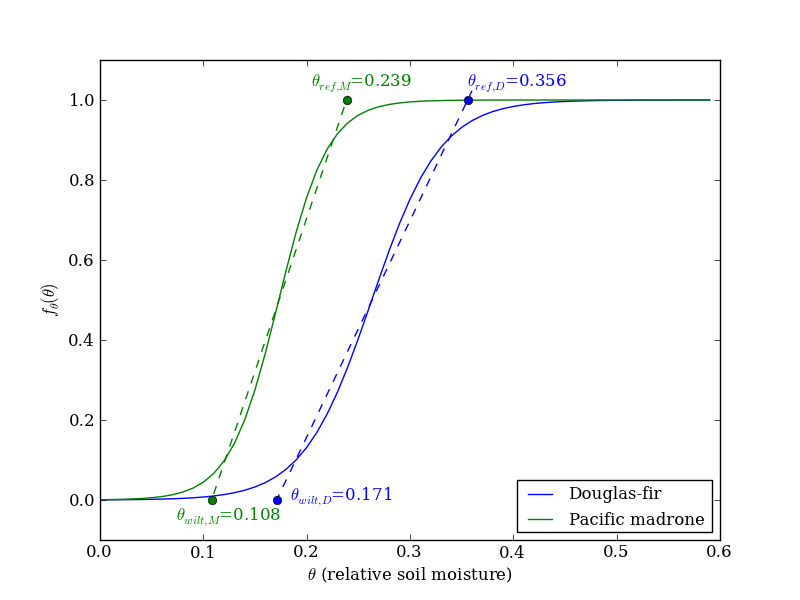
\includegraphics[width=0.9\textwidth]{ch2-BL/figures/theta_params.png}
\caption{Solid lines: sigmoid $f_{\theta}$ functions (Equation XX) for Douglas fir (blue) and Pacific madrone (green) using the species-averaged parameters from Table XX.  Dashed lines: linear regression to $f_{\theta}$ between 0.05 and 0.95.  Symbols: extrapolation of linear regression to $f_{\theta}=0$ and $1$.}
\label{fig:BL_FeddesParams}
\end{figure}


WRF-Noah is run for the all-Douglas-fir and all-Pacific-madrone cases (Tables \ref{table:BL_NoahJarvisparams} and \ref{table:BL_WRFruns}), with a range of soil moisture values (0.08, 0.1, 0.12, 0.14).  These values are equivalent to relative soil moistures of XXXX, given that the saturation moisture content of the loam soil type used in the model is 0.439 m$^3$/m$^3$.  These relative soil moisture values span the range of values observed in August at the Angelo Coast Range Reserve (Chapter \ref{c.sapflow}, Figure XX).  Soil moisture in the Coast Range test region is reset each day at midnight local time, so that the soil moisture deviates only minimally from its stated value (e.g. case vDF-sDF-0.14 has a maximum daily decline of XX m$^3$/m$^3$).
